\documentclass[../DS04.tex]{subfiles}
\graphicspath{{./figures/}}

\begin{document}

\prblm[87]{Suspension automobile}
% \subimport{/home/nora/Documents/Enseignement/Prepa/bpep/exercices/DS/suspension_automobile/}{sujet.tex}
\partie{Comportement sur un sol non plat}

\enonce{
	\noindent
	\begin{minipage}[t]{.58\linewidth}
		Dans le cadre d'un modèle simplifié de suspension, on assimile un véhicule
		à un point matériel $G$ (masse $M = \SI{1,0e3}{kg}$) repéré par sa position
    $z_G \ez$, posé sur sa suspension.

		Celle-ci est modélisée par un ressort de raideur $k = \SI{1.0e5}{N.m^{-1}}$
		et de longueur à vide $\ell_0$, associé à un amortisseur de constante
		d'amortissement $k' = \SI{4.0e3}{N.m^{-1}.s}$.

		Le véhicule se déplace à vitesse constante $V_a = \SI{50}{km.h^{-1}}$ sur
		un sol ondulé horizontal (axe $Oz$ vers le haut).

		En outre, $G$ est soumis à l'action d'un amortisseur fluide dont la force
		est de la forme $ - k' \vv{u}$ où $\vv{u}$ est la vitesse relative de ses
		deux extrémités. On admet que l'on peut donc l'écrire~:
		\[
			\vv{f} = -k' \; \dv{t}\/(z_G - z_S) \; \ez
		\]
		L'ondulation du sol est assimilée à une sinusoïde de période spatiale
		$L = \SI{2}{m}$ et d'amplitude $z_{S0} = \SI{10}{cm}$ comptée à partir de la
		ligne moyenne.

		Pour des raisons de simplicité, on supposera ici que le rayon de la roue est
		nul, c'est-à-dire que le centre $O$ de la roue suit exactement l'ondulation
		du sol ($z_O = z_S$). \textbf{On néglige également les distances OI et GJ}.

    On ne s'intéressera qu'au mouvement sur $\ez$ bien que le véhicule se
    déplace horizontalement.
	\end{minipage}
	\hfill
	\begin{minipage}[t]{.42\linewidth}
		~
		\vspace{-15pt}
		\begin{center}
			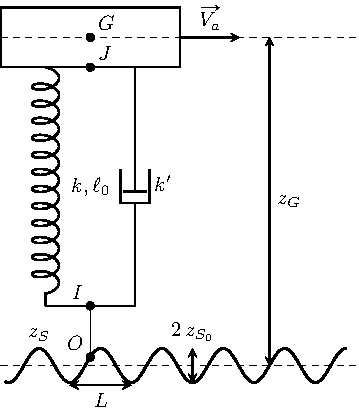
\includegraphics[width=.95\linewidth]{schema}
      \captionof{figure}{}
		\end{center}
	\end{minipage}
	\begin{tcb}(odgr){Aide aux calculs}
		\vspace{-15pt}
		\begin{gather*}
			\beforetext{\fbox{1}}
			2\pi \approx 6
			\quad~; \quad
			\frac{150}{\num{3.6}} = 42
			\\
			\beforetext{\fbox{7}}
			H (\num{4.2}) = \num{0.10}
			\\
			\beforetext{\fbox{8}}
			\num{3.3}\times \num{3.6} \approx 12
		\end{gather*}
	\end{tcb}
}

\QR{%
  \label{q:q1}
	Donner l'expression de la pulsation d'excitation $\w$ du sol en fonction de
	la vitesse $V_a$ du véhicule et de la période spatiale $L$. Justifier. Faire
	l'application numérique avec $\w$ en $\si{rad.s^{-1}}$.
}{%
  \label{q:q1}
	Si on appelle $T$ la période de l'excitation liée au sol, il faut une durée
	$T = \frac{L}{V_a}$ pour parcourir la distance $L$ qui sépare deux maxima, et
	\[
		\boxed{\w = \frac{2\pi}{T} = \frac{2\pi V_a}{L}}
		\Ra
		\xul{\w \approx \SI{42}{rad.s^{-1}}}
	\]
	\par
	Une autre manière de voir les choses~:
	\[
		z_s = z_{s0}\cos(2\pi \frac{x}{L}) =
		z_{s0}\cos(2\pi \frac{V_a}{L}t) = z_{s0}\cos(2\pi ft)
	\]
	d'où la fréquence d'excitation est $V_a/L$.
}

\QR{%
  Établir proprement le cadre d'étude. Sur quoi repose le véhicule~?
	Faire un bilan des forces pour la mise en équation du système où seront
	explicitées les forces agissant sur celui - ci. Les représenter sur un schéma.
}{%
	\begin{description}
		\item[Système] : \{châssis\} repéré par G de masse $M$~;
		\item[Référentiel] : $\Rc_{\rm sol} (O,x,y,t)$ supposé galiléen.
		\item[Repère] : $(O, \ex, \ez)$ avec $\ez$ vertical ascendant, $\ex$ dans le
		      sens de $\vv{V_a}$.
		\item[Repérage] :
      \begin{itemize}
        \bitem{Position}~: $\DS z_G \ez$
        \bitem{Vitesse}~: $\DS \zp_G \ez$
        \bitem{Accélération}~: $\DS \zpp_G \ez$
      \end{itemize}
    \item[Longueur du ressort] : $\DS \ell = z_G - z_S$
	\end{description}
	\bigbreak
  \noindent
  \begin{minipage}[t]{.65\linewidth}
	Les forces appliquées sont (cf.\ Figure~\ref{fig:sch_frc})~:
      \begin{enumerate}
      \item le poids {$\vv{P} = M\vv{g} = -Mg\ez$}~;
      \item la force élastique du ressort~:
        $\vv{F} = -k(\ell - \ell_0)\ez = -k (z_G - z_S - \ell_0)\ez$,
      \item la force de frottement fluide~:
        $\vv{f} = -k'(\zp_G - \zp_S)\ez$.
    \end{enumerate}
      \textit{Attention aux points d'application des forces et aux forces à
      prendre en compte ici~: le système étant «~le châssis~», il n'y a pas de
      réaction du support s'appliquant sur le châssis (elle s'applique à la
      roue, qui ne fait pas partie du système).}
  \end{minipage}
  \hfill
	\begin{minipage}[t]{.30\linewidth}
    ~
    \iftoggle{student}{
      \vspace{-60pt}
    }{
      \vspace{-15pt}
    }
    \begin{center}
      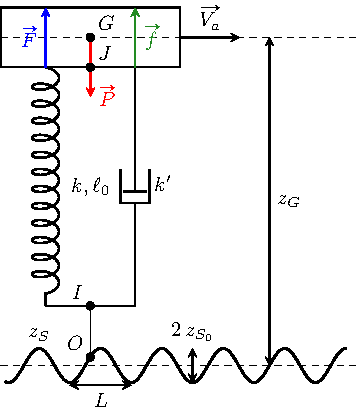
\includegraphics[width=.95\linewidth]{schema_forces}
      \captionof{figure}{}
      \label{fig:sch_frc}
    \end{center}
  \end{minipage}
}

\QR{%
	Déterminer l'équation régissant $z_{G,eq}$ la valeur de $z_G$ à l'équilibre
  pour $z_S = 0$ (route horizontale). Montrer que~:
		\[
		  z_{G,eq} = \ell_0 - \frac{Mg}{k}
		\]
}{%
	Le PFD s'écrit~:
  \begin{DispWithArrows*}
    M\vv a &= \vv F +\vv f +\vv P
    \CArrow{$\cdot \ez$}
    \\\Lra
    M\dv[2]{z_G}{t} &=
    -k(z_G - z_S - \ell_0) - Mg - k'\left(\dv{z_G}{t} - \dv{z_S}{t}\right)
    \Arrow{Équilibre}
    \\\Ra
    0 &= -k(z_{G,eq} - \ell_0) - Mg
    \Arrow{On isole}
    \\\Ra
    \Aboxed{z_{G,eq} &= \ell_0 - \frac{Mg}{k}}
  \end{DispWithArrows*}
}

\QR{%
  Exprimer l'équation différentielle vérifiée par $z = z_G - z_{G,eq}$.
  \textit{On rappelle pour cela que $z_S$ n'est pas constante.}
}{%
  Cette condition permet de simplifier l'équation précédente~:
  on pose $z = z_G - z_{G,eq}$. $z_{G,eq}$ étant constant, on en déduit
  $\dv{z}{t} = \dv{z_{G}}{t}$ et idem pour la dérivée seconde.
  On obtient finalement
  \[
    \boxed{M\zpp + k'\zp + kz = k'\zp_S + kz_S}
  \]
}

\QR{%
	Donner les expressions de la réponse complexe $\frac{\Zu}{\Zu_S}$
  ainsi que son module $\big|\frac{\Zu}{\Zu_S}\big|$ où $\Zu$ est
  l'amplitude complexe de la grandeur complexe $\zu$ associée à $z(t)$ et
  $\Zu_S$ l'amplitude complexe de celle associée à $z_S(t)$. On posera
  $x = \frac{\w}{\w_0}$.
  \par
	Montrer que~:
		\[
		  \frac{\Zu}{\Zu_S}= \frac{1 + j\frac{x}{Q}}{1 - x^2 + j\frac{x}{Q}}
		\]
	où les expressions ainsi que les valeurs numériques de $Q$ et de $\w_0$ sont
  à déterminer.
}{%
	Puisque $z_s$ varie de façon sinusoïdale, on passe en notation complexe en
  posant $\zu_S(t) = \Zu_S\exp(\jw t)$ et $\zu(t) = \Zu\exp(\jw t)$
  en RSF.

	L'équation différentielle devient, après simplification par $\exp(\jw t)$,
  \[
    -M\w^2\Zu + \jw k'\Zu + k\Zu = \jw k'\Zu_S + k\Zu_S
  \]
  d'où
  \begin{gather*}
        \frac{\Zu}{\Zu_S} =
        \frac{\jw k' + k}{k - M\w^2 + \jw k'} =
        \frac{1 + \jw \frac{k'}{k}}{1 - \frac{M\w^2}{k} + \jw \frac{k'}{k}}
        \\\Ra
        \boxed{\frac{\Zu}{\Zu_S} =
          \frac{1 + j\frac{x}{Q}}{1 - x^2 + j\frac{x}{Q}}
          \qet
          \bigg|\frac{\Zu}{\Zu_S}\bigg| =
          \sqrt{\frac{1 + \frac{x^2}{Q^2}}{(1 - x^2)^2 + \frac{x^2}{Q^2}}}
        }
  \end{gather*}
	On en déduit $\frac{k'}{k} = \frac{1}{\w_0 Q}$ et $\frac{1}{\w_0^2} =
  \frac{M}{k}$ d'où au final~:
  \[
    \boxed{\w_0 = \sqrt{\frac{k}{M}} = \SI{10}{rad.s^{-1}}}
    \qet
    \boxed{Q = \frac{\sqrt{Mk}}{k'} = \num{2.5}}.
  \]
}


\QR{%
	Tracer l'allure de $|\Hu| = \big|\frac{\Zu}{\Zu_S}\big|$ en fonction de $x$.
  Quelle est la signification physique de $|\Hu|$~?
}{%
	On a affaire à un filtre mécanique passe bas du second ordre. Un tracé sous
  python/calculatrice donne le graphique suivant en échelle linéaire (à gauche)
  ou logarithmique (à droite).
	\begin{figure}[htbp!]
		\centering
		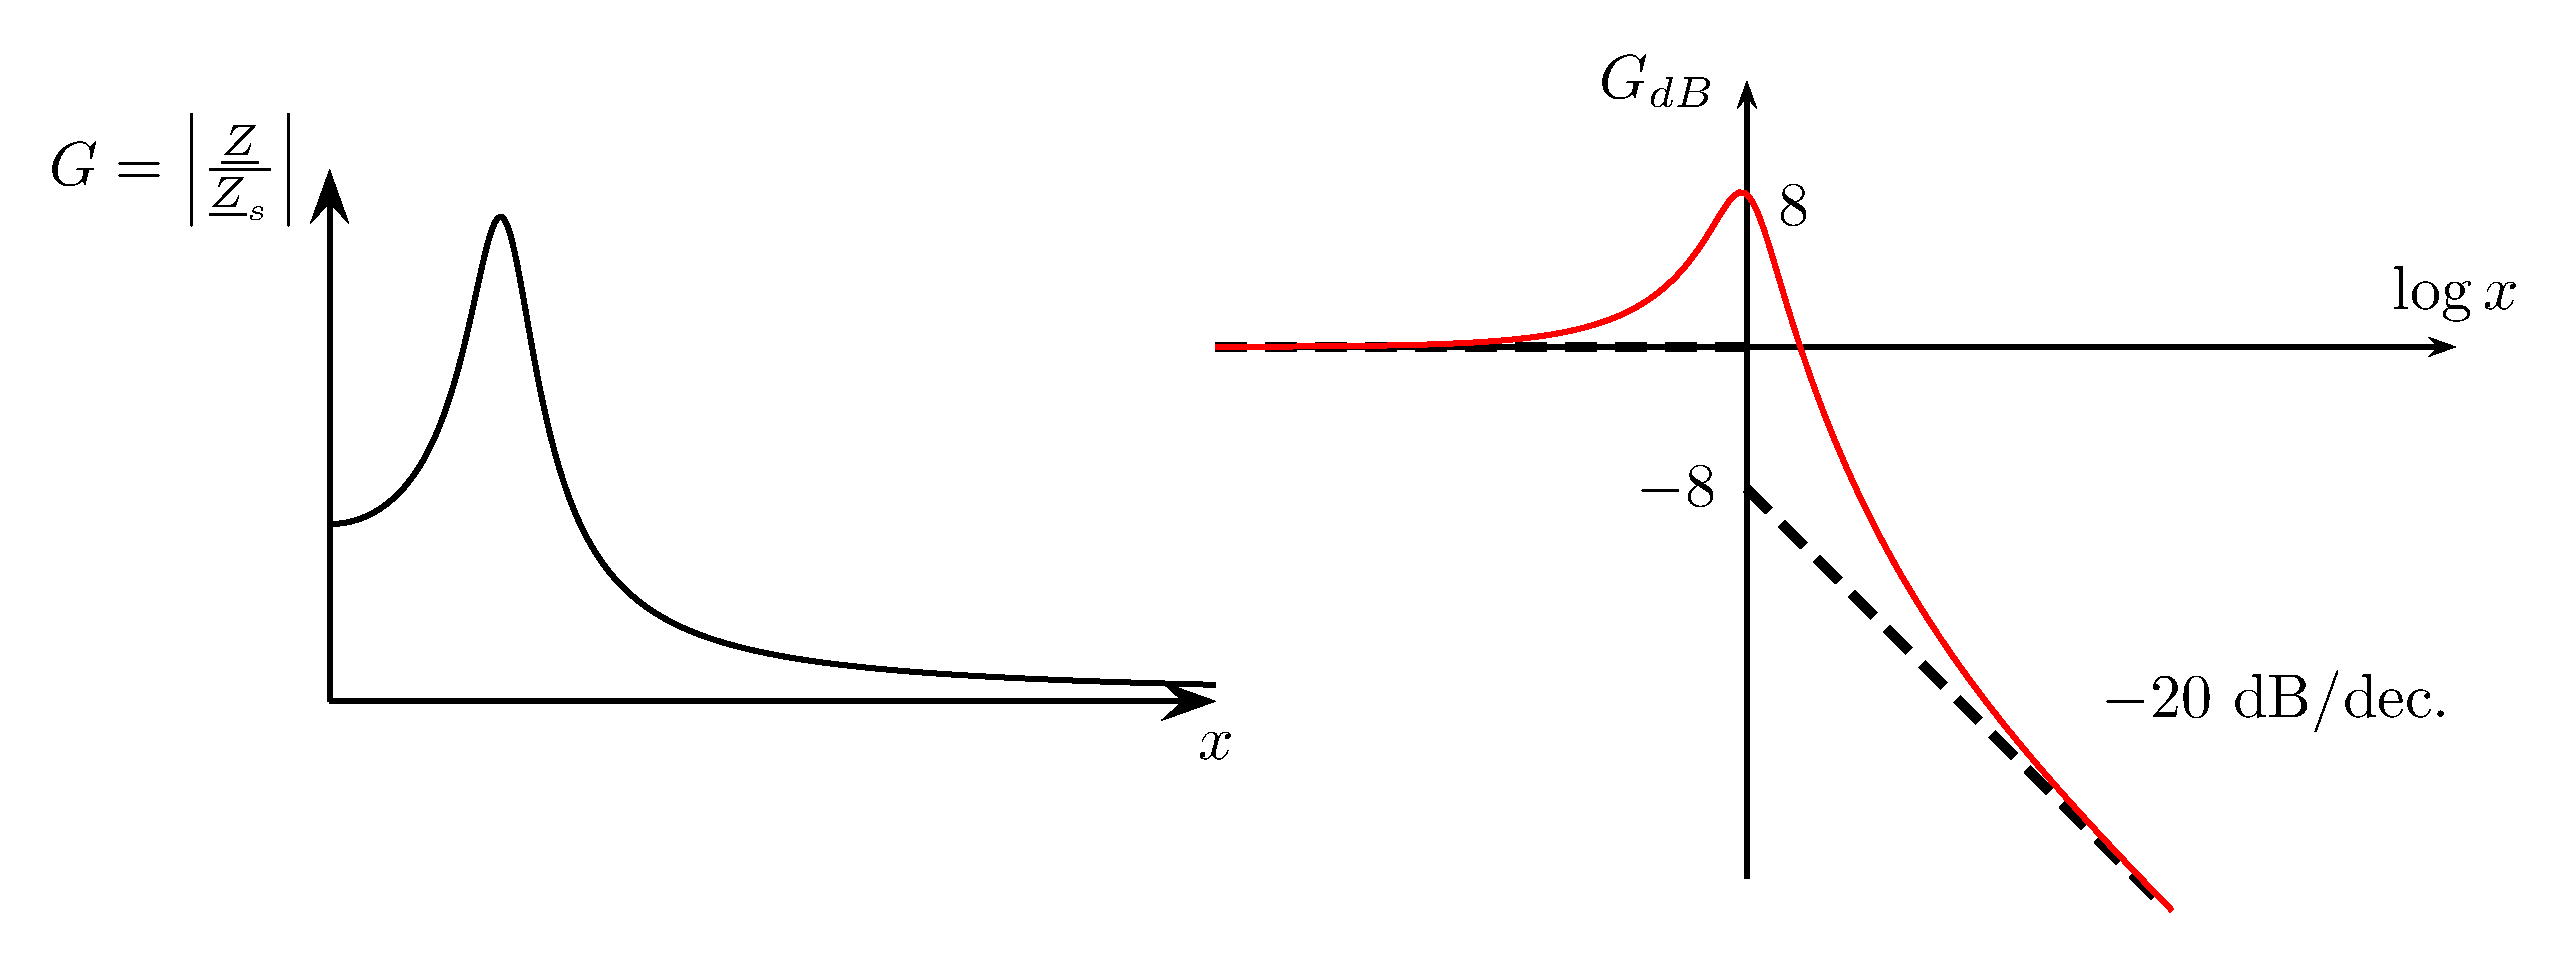
\includegraphics[width=.9\linewidth]{graphe}
    \captionof{figure}{}
	\end{figure}

	Physiquement $H = |\xul H|$ représente à quel point les perturbations de la
  route vont être amplifiées (si $H>1$) ou atténuées (si $H<1$) en fonction de
  la fréquence d'excitation (donc en partie en fonction de la vitesse du
  véhicule).
}

\QR{%
	Calculer l'amplitude des oscillations du véhicule se déplaçant à la vitesse
  $V_a$.
}{%
	Si le véhicule roule à $V_a = \SI{50}{km.h^{-1}} = \SI{13,9}{m.s^{-1}}$,
  $\w \approx \SI{42}{rad.s^{-1}}$ (pulsation des oscillations ressenties par
  læ passagærx) comme déterminé question~\ref{q:q1}. Ainsi, $x = \num{4.2}$, et
  \[
    \xul{Z = H (\num{4.2})\cdot Z_S \approx \SI{1,0}{cm}}
  \]
  (assez faible).
}

\QR{%
	À quelle(s) allure(s) ne faudrait-il surtout pas rouler sur ce sol ondulé, et
  pourquoi~? Répondre en $\si{m.s^{-1}}$ et en $\si{km.h^{-1}}$. Calculer
  l'amplitude du mouvement.
  \par
  On supposera que la valeur de $Q$ déterminée précédemment permet de répondre
  simplement.
}{%
	Il ne faut pas rouler à $V_a = V_0$ correspondant à la résonance qui a lieu
  pour $\w \approx \w_0$, soit
  \[
    V_0 \approx \frac{L\w_0}{2\pi}
    \approx \SI{3,2}{m.s^{-1}} =
    \xul{\SI{12}{km.h^{-1}}}
  \]
	Le système entrerait alors en résonance, læ passagærx ressentirait des
  oscillations d'amplitude $\DS Z(\num{10}) \approx QZ_S = \SI{25}{cm}$ et
  cela détériorerait les amortisseurs.

	\textit{Attention, ici la résonance n'a pas lieu pour $\w = \w_0$, c'est plus
  compliqué. Annoncer «~on sait que $H$ est maximum pour $x = 1$~» présente donc
  assez mal~! En pratique, $\w_r \approx \w_0$ lorsque $2Q^2 \gg 1$ ce qui est
  le cas ici ($Q = 2,5$).}
}

\QR{%
	À la lueur des résultats obtenus, proposer un moyen de ralentissement des
  véhicules à l'entrée des zones urbaines, limitant la vitesse d'entrée à
  $\SI{60}{km.h^{-1}}$.
}{%
	En plaçant des bandes rugueuses à une distance $L_0$ bien choisie, on peut,
  en admettant que la fréquence de résonance est la même pour tous les
  véhicules, s'arranger pour que $V_0$ soit légèrement supérieure à la vitesse
  limite de $\SI{50}{km.h^{-1}}$ en zones urbaines, soit par exemple
  $\SI{60}{km.h^{-1}}$~:
  \begin{gather*}
    \w_0 = \frac{2\pi V_0}{L_0}
    \Lra
    \boxed{L_0 = \frac{2\pi V_0}{\w_0}}
    \qav
    \left\{
    \begin{array}{rcl}
      2\pi & \approx & 6
      \\
      V_0 & = & \SI{60}{km.h^{-1}} =
      \SI[parse-numbers=false]{\frac{60}{3.6}}{m.s^{-1}}
      \\
      \w_0 & = & \SI{10}{rad.s^{-1}}
    \end{array}
    \right.\\
    \AN
    \xul{
      L_0 = \SI{10}{m}
    }
  \end{gather*}
}

\partie{Comportement lors du franchissement d'une bordure}

\enonce{
	\noindent
	\begin{minipage}[t]{.49\linewidth}
    On s'intéresse maintenant au cas du franchissement d'une bordure
    (le niveau du sol s'élève brusquement) avec $z_S(t) = 0~\forall t <0$ et
    $z_S(t) = z_0~\forall t>0$ (échelon d'altitude).
    \par
    Cette fonction n'est ni dérivable, ni continue en $t = 0$ et on ne pourra
    ainsi pas résoudre simplement l'équation mécanique obtenue dans la partie
    précédente.
    \smallbreak
		On se propose alors d'étudier le régime transitoire correspondant au
    franchissement de la bordure à l'aide d'un circuit électrique équivalent,
    c'est-à-dire régi par une équation différentielle similaire.
		\par
		Le circuit ci-contre est alimenté par un générateur de tension parfait
    délivrant une tension sinusoïdale $\uu_e$ de pulsation $\w$. On cherche
    dans un premier temps à identifier la tension qui correspondra à
    l'inconnue $z(t)$ du problème mécanique.
	\end{minipage}
	\hfill
	\begin{minipage}[t]{.49\linewidth}
    ~
    \vspace{-15pt}
		\begin{center}
			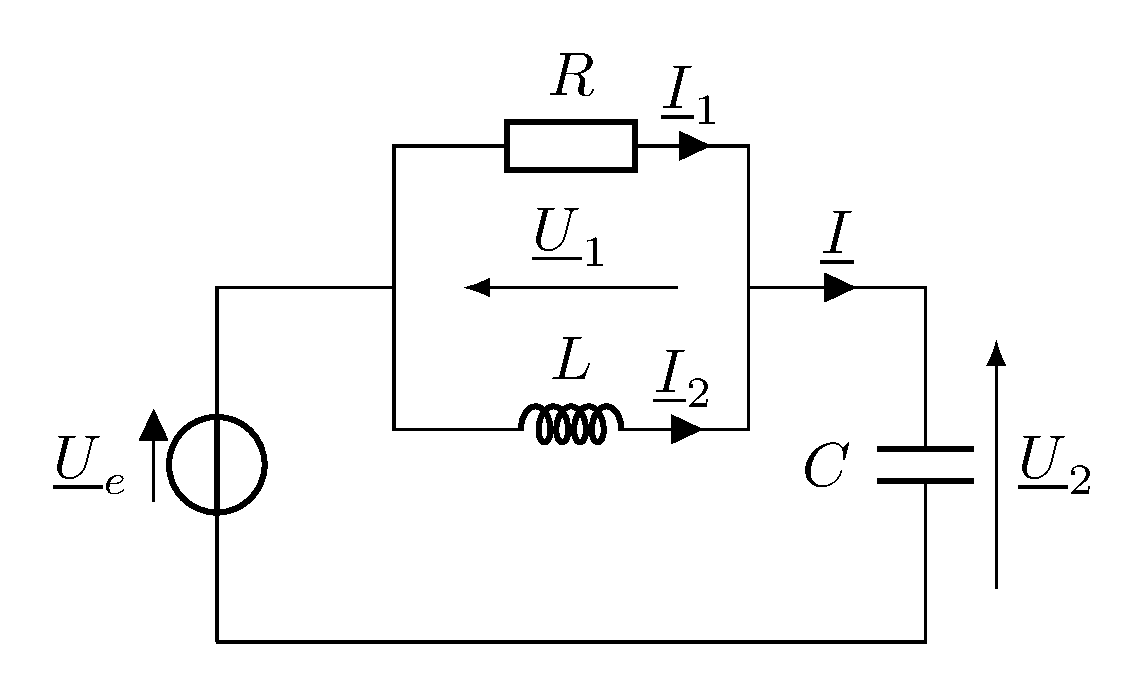
\includegraphics[width=\linewidth]{circuit}
      \captionof{figure}{Circuit électrique équivalent.}
		\end{center}
	\end{minipage}
}

\QR{%
	Déterminer l'impédance équivalente $\Zu$ de ce circuit vue depuis le
  générateur. L'écrire sous la forme $\frac{1}{\jcw}$ multipliant une fraction
  de 2 expressions adimensionnées, sans chercher à faire apparaître des
  constantes $w_0$ ou $Q$.
}{%
	Vue du générateur, l'impédance est un condensateur en série avec (une
  résistance et une bobine en parallèle). D'où
  \begin{DispWithArrows*}
    \Zu &=
    \frac{1}{\jcw} + \frac{\jj RL\w}{R + \jlw}
    \Arrow{Même dénominateur}
    \\\Lra
    \Zu &=
    \frac{R + \jlw - RLC\w^2}{jC\w(R + \jlw)}
    \Arrow{On factorise par $R$}
    \\\Lra
    \Aboxed{
      \Zu &= \frac{1 + \jj \frac{L}{R}\w - LC\w^2}{\jcw(1 + \jj \frac{L}{R}\w)}
    }
  \end{DispWithArrows*}
}

\QR{%
	Par une analyse du comportement à basses et hautes fréquences, quelle grandeur
  de sortie $\Uu_s$ doit être choisie (parmi $\Uu_1$ ou $\Uu_2$) pour obtenir
  une fonction de transfert harmonique équivalente à celle de la suspension
  automobile \{ $M$, $k$, $k'$ \} sur une route déformée
  sinusoïdalement, c'est-à-dire que~:
	\begin{align}
		\label{eq:ft}
		\frac{\Uu_s}{\Uu_e} = \frac{1 + \jj \frac{x}{Q}}{1 - x^2 + \jj \frac{x}{Q}}
	\end{align}
	où $x = \frac{\w}{\w_0}$ est la pulsation réduite~; $\w_0$ une pulsation
  propre et $Q$, le facteur de qualité. Déterminer alors les expressions de ces
  constantes en fonction de $R$, $L$ et $C$.
}{%
	Deux choix sont possibles et dans les deux cas, on va vérifier les
  comportements asymptotiques~:
	\begin{itemize}
		\item pour $u_s = u_1$, on a $\Uu_1 \to 0$ quand $\w \to 0$ (car la bobine
      est équivalente à un fil en BF) et ce résultat n'est pas compatible avec
      la fonction de transfert attendue (réponse non nulle en basse fréquence).
		\item pour $u_s = u_2$, on a $\Uu_2 \to 0$ quand $\w \to +\infty$
      (condensateur équivalent à un fil en HF) puis $\Uu_2 \to \Uu_e$ quand
      $\w \to 0$ (tension nulle aux bornes de la bobine + loi des mailles). Ce
      comportement asymptotique est compatible avec celui du filtre proposé dans
      la partie précédente.
	\end{itemize}
	On retient ainsi pour la suite $u_s = u_2$ et on obtient la fonction de
  transfert en utilisant la formule du pont diviseur de tension~:
  \[
    \frac{\Uu_s}{\Uu_e} =
    \frac{\frac{1}{\jcw}}{\Zu(\w)} =
    \frac{1}{\frac{1 + \jj \frac{L}{R}\w - LC\w^2}{1 + j\frac{L}{R}\w}}
    \Lra
    \boxed{
      \frac{\Uu_s}{\Uu_e} = 
        \frac{1 + j\frac{L}{R}\w}{1- LC\w^2 + j\frac{L}{R}\w}
    }
  \]
  En identifiant à la forme proposée par l'énoncé on obtient
  \[
    \w^2/\w_0^2 = LC\w^2
    \Ra 
    \boxed{\w_0 = \frac{1}{\sqrt{LC}}}
    \qqet
    \frac{\w}{Q\w_0} =\w \frac{L}{R}
    \Ra 
    \boxed{Q = \frac{R}{L\w_0} = R\sqrt{\frac{C}{L}}}
  \]
	\textit{L'expression du facteur de qualité n'est pas la même que celle
  obtenue pour le circuit RLC série. Cependant, elle est bien sans dimension.}
}

\QR{%
	En comparant les expressions obtenues dans les deux modélisations (mécanique
  et électrique), proposer des équivalences électromécaniques. Attention, ce ne
  sont pas forcéments les équivalences classiques du RLC série.
}{%
	$\w_0 = \frac{1}{\sqrt{LC}}$ en électrique et $\w_0 = \sqrt{\frac{k}{M}}$
  d'un coté, et de l'autre coté  $Q = R\sqrt{\frac{C}{L}}$ et
  $Q = \frac{1}{k'}\sqrt{Mk}$.
  \par
	Vu la forme de $\w_0$, on est amené à proposer naturellement
  $(k = \frac{1}{L}~; M = C)$ ou  $(k = \frac{1}{C}~; M = L)$ toutefois, du
  côté de $Q$, les grandeurs qui «~passent du dénominateur dans $\w_0$ au
  numérateur dans $Q$~» sont $M$ et $C$.
  \par
	Il parait donc raisonnable de proposer
  \[
    \boxed{
      M\lra C
      \quad ; \quad 
      k\lra \frac{1}{L}
      \quad ; \quad 
      k'\lra\frac{1}{R}
    }
  \]
  (et bien sûr $U_s = z_v$ et $U_e = z_s$)
  \par
	\textit{D'autres relations d'équivalences pourront être obtenues lors de
  l'étude d'autres circuits électriques. Ces résultats ne sont donc pas à
  apprendre par cœur.}
}

\QR{%
	Montrer que l'équation différentielle reliant $u_s(t)$ ($u_1$ ou $u_2$) à
  $u_e(t)$ et aux données du problème s'écrit~:
  \[
    \dv[2]{}{t}u_s + \frac{1}{RC} \dv{}{t}u_s + \frac{1}{LC}u_s =
    \frac{1}{RC} \dv{}{t} u_e + \frac{1}{LC} u_e
  \]
	avec $u_e(t)$ la tension aux bornes du générateur non constante.
}{%
  Avec la loi des mailles~:
  \[
    u_e = u_1 + u_2 \Lra u_1 = u_e - u_2
  \]
  \begin{isd}
      On cherche à simplifiser $u_1$. On a pour ça~:
    \begin{DispWithArrows*}[fleqn, mathindent=2pt]
      i &= i_1 + i_2
      \Arrow{$i_1 = \frac{u_1}{R}$}
      \\\Lra
      i &= \frac{u_1}{R} + i_2
      \CArrow{$\dv{t}$}
      \\\Ra 
      \dv{i}{t} &= \frac{1}{R}\dv{u_1}{t} + \dv{i_2}{t}
      \Arrow{$u_1 = L \dv{i_2}{t}$}
      \\\Lra
      \dv{i}{t} &= \frac{1}{R} \dv{u_1}{t} + \frac{1}{L}u_1
      \Arrow{On isole $u_1$}
      \\\Lra
      \Aboxed{u_1 &= L \dv{i}{t} - \frac{L}{R}\dv{u_1}{t}}
      \Arrow{$i = C \dv{u_2}{t}$}
      \\\Lra
      u_1 &= LC \dv[2]{u_2}{t} - \frac{L}{R} \dv{u_1}{t}
      \Arrow{$u_1 = u_e - u_2$}
      \\\Lra
      \Aboxed{u_1 &= LC \dv[2]{u_2}{t} - \frac{L}{R}\left( \dv{u_e}{t} -
      \dv{u_2}{t} \right)}
    \end{DispWithArrows*}
    \tcblower
  Ainsi, dans la loi des mailles~:
  \begin{DispWithArrows*}[fleqn, mathindent=2pt, groups]
    u_1 &= u_e - u_2
    \Arrow{On injecte $u_1$}
    \\\Lra
    LC \dv[2]{u_2}{t} + \frac{L}{R} \dv{u_2}{t} - \frac{L}{R} \dv{u_e}{t}
        &= u_e - u_2
    \Arrow{On regroupe}
    \\\Lra
    LC \dv[2]{u_2}{t} + \frac{L}{R} \dv{u_2}{t} + u_2
        &= \frac{L}{R} \dv{u_e}{t}
    + ue
    \Arrow[new-group]{$\times \frac{1}{LC}$}
    \\\Lra
    \Aboxed{
      \dv[2]{u_2}{t} + \frac{1}{RC} \dv{u_2}{t} + \frac{1}{LC} u_2 &=
      \frac{1}{RC} \dv{u_e}{t} + \frac{1}{LC} u_e
    }
  \end{DispWithArrows*}
  \end{isd}
   On aurait aussi pu partir de la fonction de transfert obtenue précédemment~:
   \begin{DispWithArrows*}
      \frac{\Uu_2}{\Uu_e} &= \frac{1+\jj \frac{x}{Q}}{1+(\jx)^{2} + \jj
      \frac{x}{Q}}
      \Arrow{On isole}
      \\\Lra
      \Uu_2 \left(1 + \left(\frac{\jw}{\w_0}\right)^{2} +
          \frac{\jw}{w_0Q}\right) &=
      \Uu_e \left(1 + \frac{\jw}{w_0Q}\right)
      \Arrow{En réels}
      \\\Lra
      \frac{1}{w_0{}^{2}}\dv[2]{u_2}{t} + \frac{1}{w_0Q} \dv{u_2}{t} + u_2
                                  &=
      u_e + \frac{1}{w_0Q}\dv{u_e}{t}
      \CArrow{$\times \w_0{}^{2}$}
      \\\Lra
      \Aboxed{
        \dv[2]{u_2}{t} + \frac{\w_0}{Q} \dv{u_2}{t} + \w_0{}^{2}u_2
                                              &=
        \frac{\w_0}{Q}\dv{u_e}{t} + \w_0{}^{2}u_e
      }
   \end{DispWithArrows*}
   Ce qui est bien la même chose en devéloppant et $\w_0$ et $Q$.
}

\enonce{
	\bigskip
	Pour l'étude du régime transitoire associé au franchissement de la bordure,
  on considère la fonction échelon
		\[
		  u_e:t \mapsto 0,~\forall t \le 0
      \qqet
      u_e:t \mapsto E,~\forall t >0
		\]
	Dans toute la suite, on raisonnera sur les équations faisant intervenir des
  grandeurs $\w_0$ et $Q$ afin de pouvoir relier aisément le système mécanique
  au système électrique.
	\bigskip
}

\QR{%
	En quoi le choix pour $u_e$ est-il pertinent pour la description du
  franchissement d'une bordure~?
}{%
	Dans le cadre de l'analogie électromécanique, la tension $u_e$ aux bornes du
  GBF est analogue à la hauteur du sol $z_s$. Lors du franchissement d'un
  trottoir, la hauteur (constante avant) va ainsi soudainement augmenter d'une
  dizaine de centimètres puis redevenir constante. C'est bien le comportement
  qui est décrit ici.
}


\QR{%
	Obtenir deux conditions initiales sur $u_s$ en $t = 0^+$. Une réponse
  rigoureusement rédigée est attendue. Exprimez ensuite ces dernières à l'aide
  de $E$, $\w_0$ et $Q$.
}{%
	La charge initiale du condensateur n'est pas mentionnée dans l'énoncé. À
  $t = 0^-$, on a $i(0^-) = 0$ (condensateur en RP) puis $u_1(0^-) = 0$
  (bobine $\lra$ fil en RP) donc $i_1(0^-) = 0$ (résistance) et finalement
  $i_2(0^-) = 0$ (loi des nœuds).
  \smallbreak
	On en déduit à l'aide de la loi des mailles appliquées à $t = 0^-$ que
  $0 = 0 + u_2(0^-) \Rightarrow u_2(0^-) = 0$ or la tension aux bornes du
  condensateur est continue donc $\boxed{u_2(0^+) = 0}$.
  \bigbreak
	La dérivée de cette tension n'est pas nécessairement continue (aucun résultat
  de cours ne permet de le prouver rapidement). On va donc étudier le circuit à
  $t = 0^+$ en y appliquant la loi des mailles~: $E = u_1(0^+) + u_2(0^+)
  \Rightarrow u_1(0^+) = E$. De plus, on a par continuité du courant à travers
  la bobine, $i_2(0^+) = i_2(0^-) = 0$ mais aussi $i_1(0^+) = u_1(0^+)/R = E/R$.
	\\
	Finalement, l'application de la loi des nœuds donne $i(0^+) = i_1(0^+) = E/R
  = C \dv{u_2}{t}(0^+) \Rightarrow \boxed{\dv{u_2}{t}(0^+) = \frac{E}{RC} =
  \frac{E \w_0}{Q}}$
}

\QR{%
  Résoudre ensuite l'équation différentielle obtenue pour $t>0$ (on retiendra la
  valeur du facteur de qualité obtenue dans la première partie).
}{%
  Pour $t>0$, on a $u_e(t) = E$ et donc~:
	\[
	  \dv[2]{}{t}u_2 + \frac{\w_0}{Q} \dv{}{t}u_2 + \w_0^2 u_2 = \w_0^2 E
	\]
  Pour $Q = 2,5 > 1/2$, on se place dans le cas du régime pseudo-périodique et
  donc
	\[
	  u_2(t) = e^{- t/\tau} \pa{A \cos (\W t) + B \sin(\W t)} + E
	\]
  avec $\W = \frac{\w_0}{Q}\sqrt{4Q^{2} - 1}$ et $\tau = \frac{\w_0}{2Q}$.
  La première CI donne $A +E= 0$. On dérive ensuite la tension~:
  \[
    \dv{u_2}{t}(t) =
      - \frac{1}{\tau}e^{-t / \tau} ( B \sin(\W t) - E \cos(\W t))
      + e^{-t \tau} (B \W \cos(\W t) +E \sin(\W t))
  \]
  La deuxième CI donne $\frac{E\w_0}{Q} = \frac{2E}{\tau} =\frac{E}{\tau} + B\W
  \Rightarrow B = \frac{E}{\tau \W}$.
  On trouve au final~:
  \[
    \boxed{
      u_2(t) = E e^{-t/\tau}\pa{ \frac{E}{\tau \W}\sin(\W t) -  \cos(\W t)} + E
    }
  \]
}

\QR{%
	Représenter sur un même graphique la solution obtenue pour la valeur du
  facteur de qualité trouvée précédemment, ainsi que pour $Q = 0,51$ et
  $Q = 10$. On prendra soin de déterminer la valeur de la période et/ou du
  temps de réponse pour chaque graphique, sans chercher à démontrer les
  expressions utilisées.
	\\
	Pour les applications numériques, on prendra $E=\SI{1}{V}$ et
  $\w_0 = \SI{10}{rad.s^{-1}}$.
}{%
	\begin{figure}[htbp!]
		\centering
		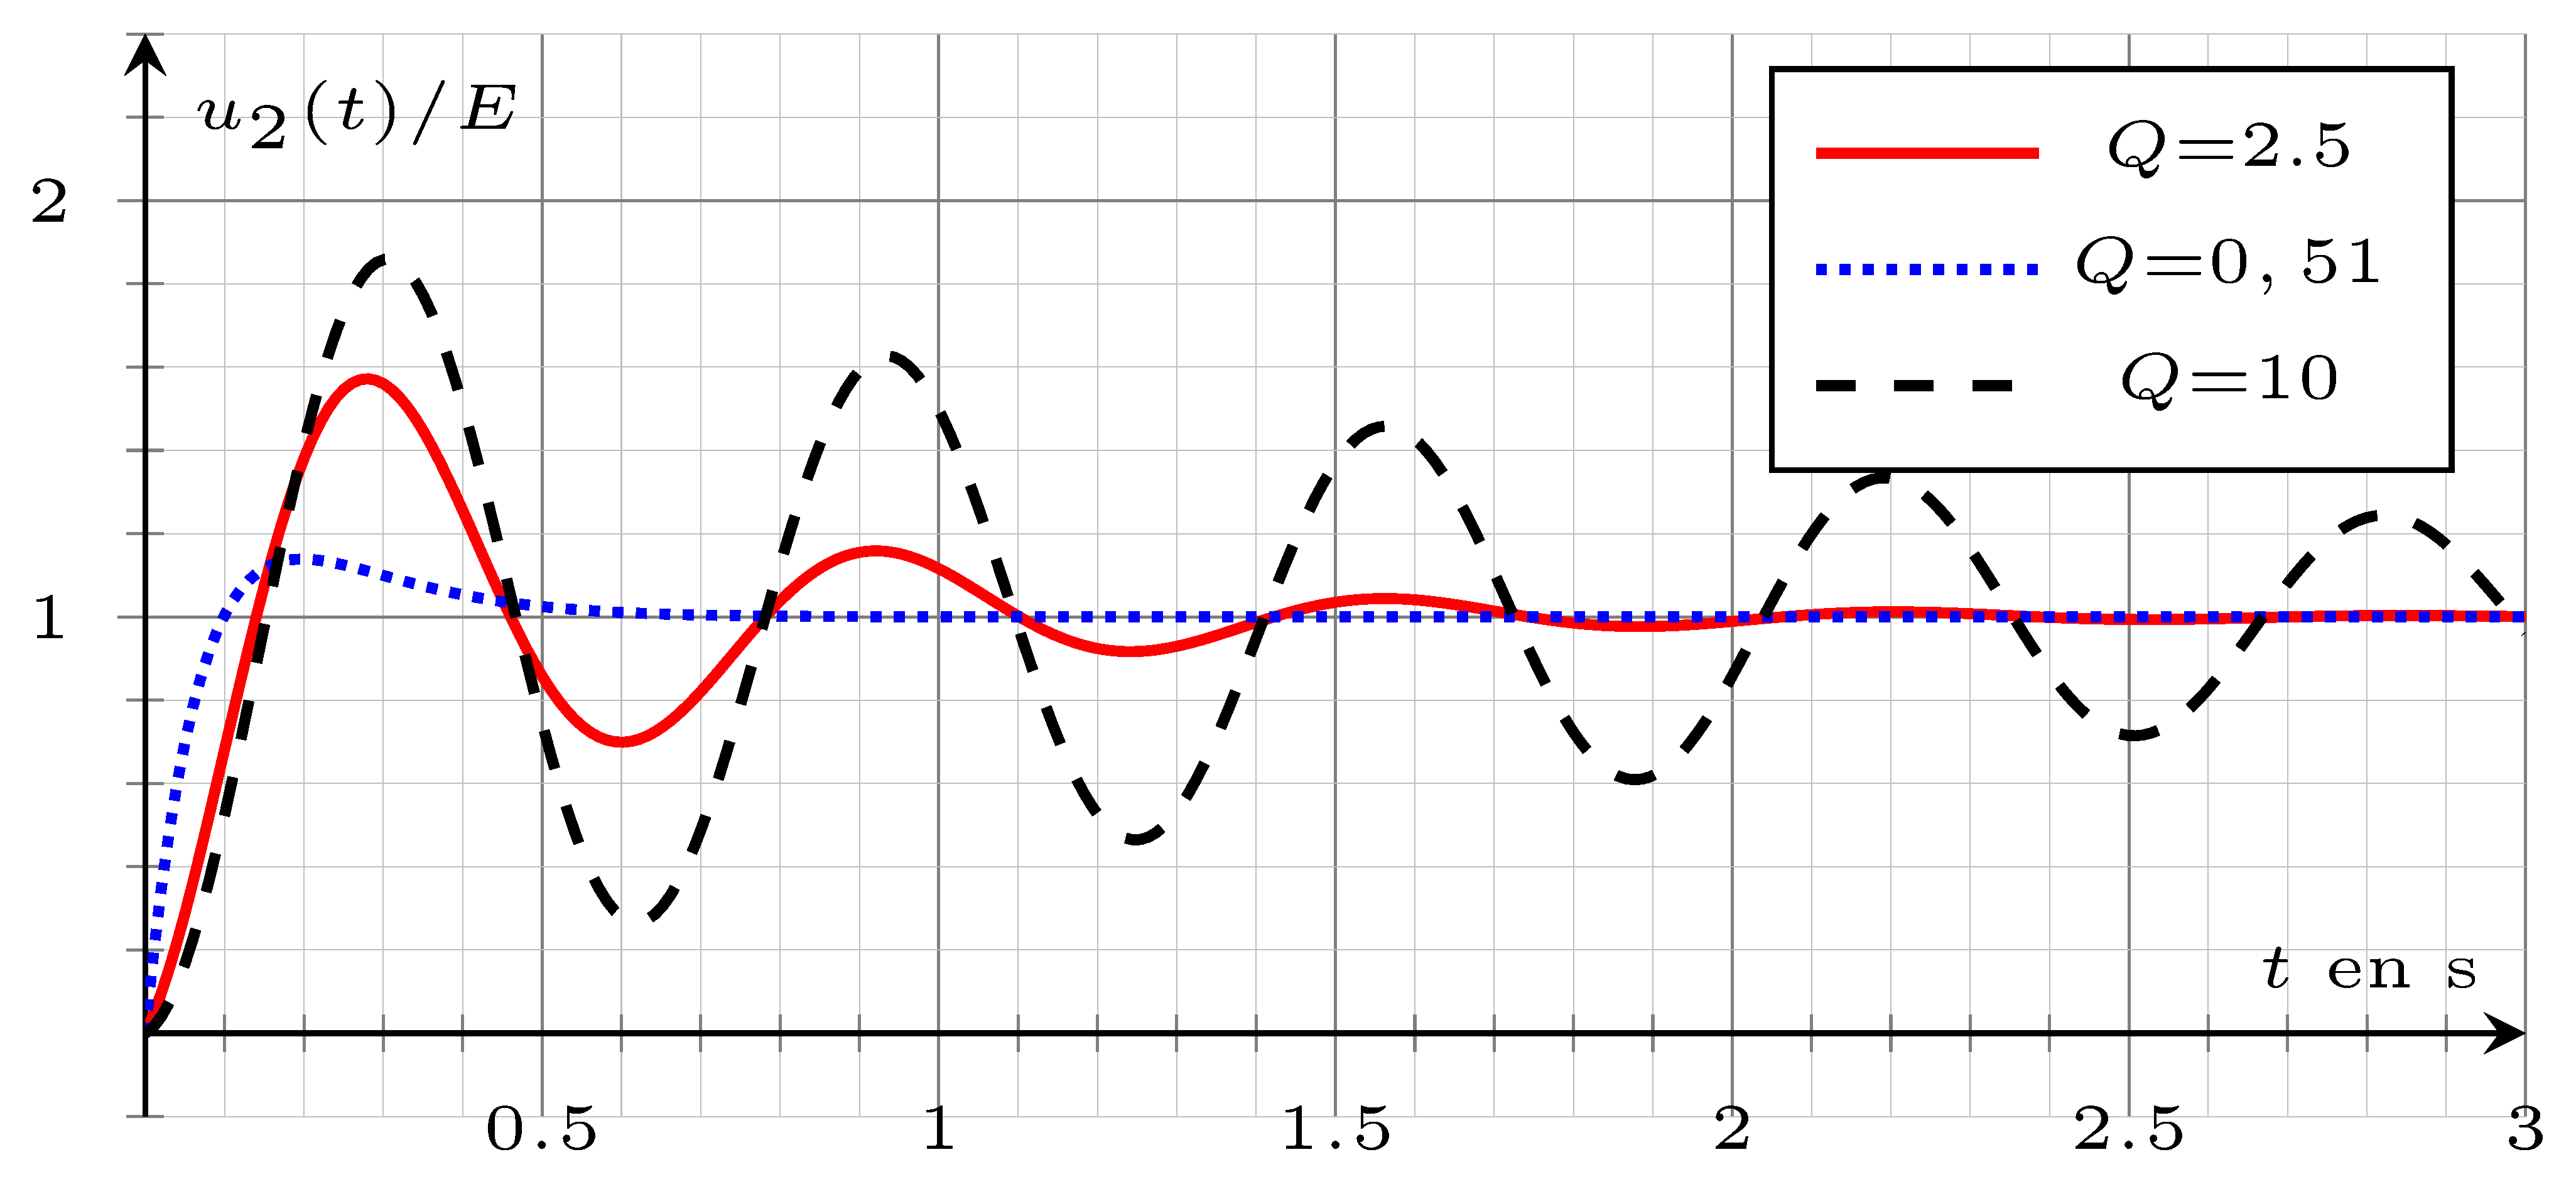
\includegraphics[width=.9\linewidth]{transitoire}
    \captionof{figure}{}
	\end{figure}

	Graphiquement, on obtient $u_{2,\rm max }(Q = 10) = 1,95E$,
  $u_{2,\rm max }(Q = 2.5) = 1,6E$ puis finalement $u_{2,\rm max }(Q = 0,51)
  \approx 1,15 E$ (peu de dépassement dans le dernier cas).
}

\subsection{Conclusion}

\QR{%
	Afin de construire un système de suspension efficace, que préconisez-vous pour
  le choix du facteur de qualité au regard des résultats obtenus dans les
  précédentes parties~?
}{%
	Dans le premier cas (sol ondulé), on constate que pour un facteur de qualité
  élevé, on peut rencontrer un phénomène de résonance qui peut être génant.
  Dans le deuxième cas (franchissement d'une bordure), on observe aussi que le
  dépassement dépend du facteur de qualité.
	\par
	\medskip
	Il convient donc de réaliser un système avec un \textbf{faible facteur de
  qualité}, dans la limite du raisonnable~: il ne faut pas non plus que les
  amortisseurs soient rigides. Une valeur autour de \num{0.5} paraît appropriée.
}

\end{document}
